\chapter{Описание разработанного метода}

\section{Общий обзор}
В данном разделе мы опишем общую идею разработанного метода.

\subsection{Входные данные}
На входе PDB, в каком виде данные. единицы измерения
(полстраницы, возможно, с картинкой)
\vspace{10cm}

\subsection{Общие соображения}
Включим в состав множества протяженных регионов, содержащих ,,энергетически горячие аминокислотные остатки'', следующее:
\begin{itemize}
\item аминокислоты, образующие ,,интерфейс'' взаимодействия с парной цепочкой или белком (с использованием отсечки по расстоянию от второй цепочки)
\item аминокислоты, образующие поверхность ,,карманов'', находящихся в области взаимодействия пары белков
\item не-гидрофобные аминокислоты, являющиеся соседними по отношению к аминокислотам, образующим интерфейс
\item если интерфейс взаимодействия образован петлями, то добавим все аминокислоты, образующие петли 
\end{itemize}

\section{Детальное описание}
В данном разделе мы дадим исчерпывающее описание алгоритма вместе с необходимыми для реализации деталями.
\subsection{Построение графа}
\begin{itemize}
\item Рассматриваем одновременно 2 цепочки, образующие белковый комплекс.
\item Начнем с построения выпуклой оболочки и триангуляции Делоне для каждой из них, будем искать протяженные регионы с энергетически горячими аминокислотными остатками  на одной из них. Строить будем по центрам атомов, формирующих аминокислоты цепочки.
\item Выберем все треугольники выпуклой оболочки, в которых хотя бы одна вершина удалена от некоторых атомов второй цепочки не далее, чем на выбранное (фиксированное) значение отсечки.
\end{itemize}


\begin{itemize}
\item Берется структура в PDB.
\item Центры атомов рассматриваются как точки. По ним строится триангуляция Делоне (с помощью scipy.delaunay - обертки над алгоритмом qhull).
\item Берется невзвешенная триангуляция -- по тем же соображениям, по которым она используется в CAVER (эвристика).
\end{itemize}
Я сопоставляю графу триангуляцию по тому же принципу, как в статье по CAVER:

\begin{center}
\resizebox{!}{0.3\textheight}{
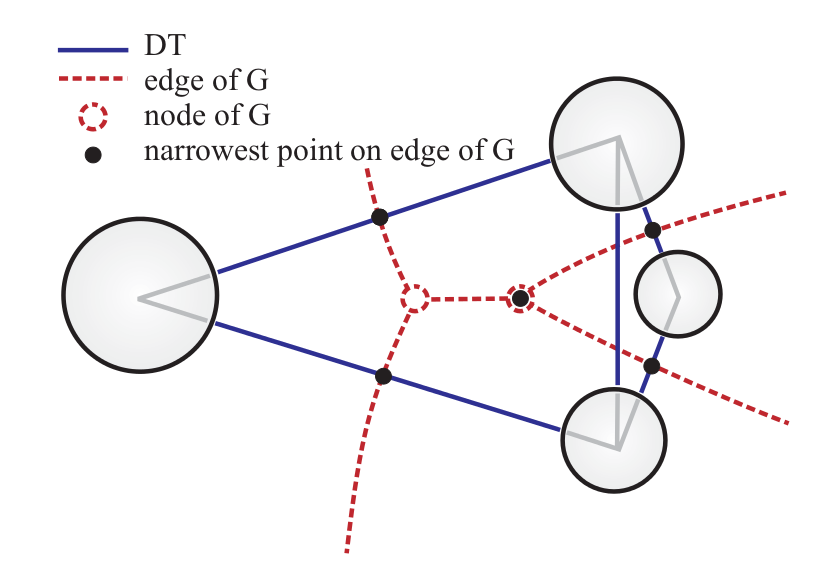
\includegraphics{image4_caver.png}
}

[Computation of tunnels in protein molecules using
Delaunay triangulation, P.Medek, et al., 2007]
\end{center}

Треугольники триангуляции -- вершины графа, ребра графа -- общие стороны треугольников (с ограничением снизу на длину).

Дополнительно используется такой же граф по треугольникам выпуклой оболочки (без ограничения снизу на длину стороны, просто по смежным по стороне треугольникам).

Выбирается начальное множество треугольников выпуклой оболочки. Сейчас берутся треугольники, вершины которых недалеко (в смысле отсечки по расстоянию) от второго белка.

\subsection{Псевдо-интерфейс}
\begin{itemize}
\item определяем множество треугольников выпуклой оболочки, для которых хотя бы одна вершина удалена от центров атомов второй цепочки не больше, чем на выбранное значение отсечки
\item Далее расширяем интерфейс
\begin{itemize}
\item шаг 1: добавляем к интерфейсу все треугольники выпуклой оболочки, содержащие атомы аминокислот, которые уже туда попали
\item шаг 2: продлеваем регион до границы гидрофобности
\item шаг 3: продлеваем регион за границы гидрофобности на 1 аминокислоту.
\end{itemize}
\end{itemize}


В результате у нас есть одна или нескольких протяженных связных областей выпуклой оболочки, по которым можно восстановить аминокислоты.
\subsection{Поиск карманов}
\begin{itemize}
\item Начинаем с множества отобранных треугольников выпуклой оболочки (черным цветом)
\item Ищем в ширину с ограничениями
\item Ходим только по тем треугольникам, для которых ближайший треугольник выпуклой оболочки -- один из отобранных треугольников выпуклой оболочки, а не какой-либо из других треугольников выпуклой оболочки.
\item Ближайший треугольник == в смысле расстояния до ближайшей из вершин он ближе, чем другие треугольники выпуклой оболочки
\end{itemize}
\subsection{Расширение интерфейса. Добавление петель}
Почему имеет смысл добавлять петли

Перед добавлением петель треугольники триангуляции преобразуются в фрагменты последовательности аминокислот, продлеваем их, используя информацию о вторичной структуре.


\begin{itemize}
\item Сейчас вторичная структура определяются на основе вывода DSSP (biopython же).

\item Я беру непрерывные фрагменты структуры, которые не определяются как альфа-спирали или бета-листы, выбираю среди них те, в которые попадает какая-либо аминокислота, ну и добавляю их к выделяемому контуру - технической сложности никакой. Содержательности - тоже :(


\end{itemize}


\begin{itemize}
\item Я отправляла статью про петли. Что там происходит: взята ASEdb, рассмотрены короткие фрагменты петель, содержащие энергетически горячие аминокислоты и приведена их какая-то классификация.

вариантов 2: либо не добавлять петли целиком, вместо этого добавлять только такие фрагменты (в статье они приведены), либо как-то их отмечать на выделенных петлях + отмечать на удаленных петлях, которые в выделенный регион не попали.

\item про hmm думаю, напишу через пару дней.

\item вообще если получится, я разберусь как считать взвешенную триангуляцию Делоне и с помощью нее искать карманы.

\item Еще хочу почитать про O-кольца.

\end{itemize}
